\documentclass[border=6pt]{standalone}
\usepackage{garamondx}
\usepackage{pgfplots}
\usepackage{tikz}
\usepgfplotslibrary{units}
\usepackage{xcolor}
\definecolor{redtea}{rgb}{0.6823529412,0.2792156863,0.2666666667}
\usepackage{siunitx}
\usepackage{changepage}
\usepackage{calc}
\pgfplotsset{samples}
\usepgfplotslibrary{fillbetween}
\usetikzlibrary{backgrounds}
\pgfdeclarelayer{bg}
\pgfdeclarelayer{fg}
\pgfsetlayers{bg,main,fg}
\usetikzlibrary{patterns}

\pgfplotsset{compat=1.18}

\begin{document}
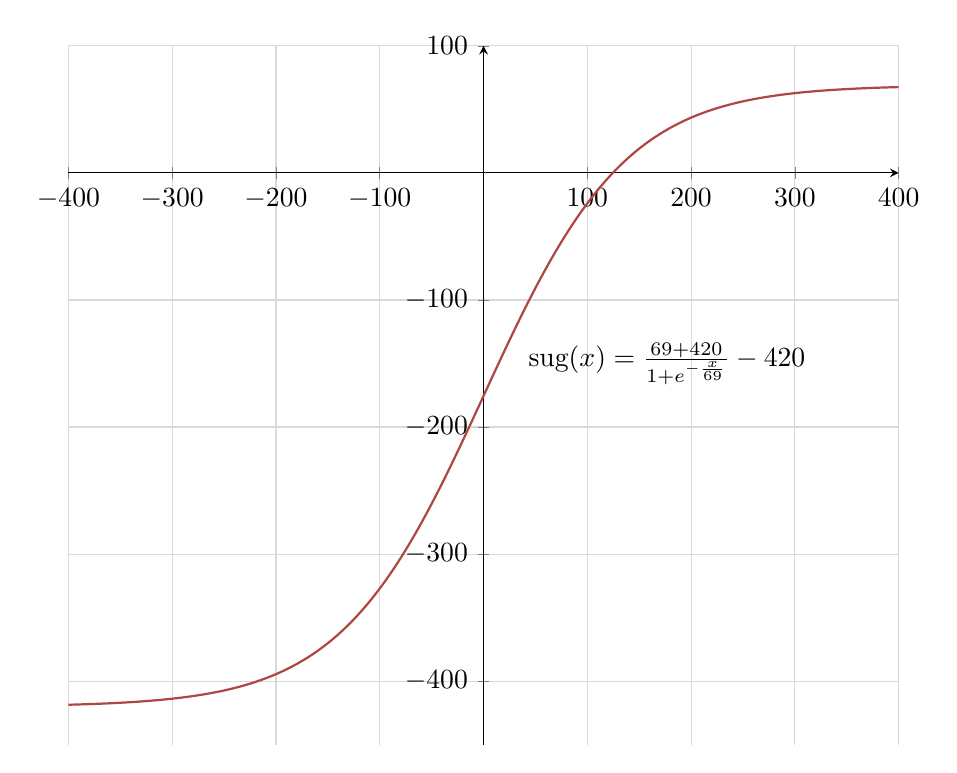
\begin{tikzpicture}
\begin{axis}[
width=\linewidth,
grid=major,
grid style={gray!30},
axis lines=middle,
xmax=400,
xmin=-400,
ymin=-450,
ymax=100,
%xtick={},
%xticklabels={}
]
\addplot [redtea, thick, smooth, domain=-400:400, restrict y to domain=-450:100, samples=1000] {((69+420)/(1+exp(-1*(x/69))))-420} node [black, left, xshift=-3em, yshift=-10em] {$\text{sug}(x)=\frac{69+420}{1+e^{-\frac{x}{69}}}-420$};
\end{axis}

\end{tikzpicture}
\end{document}
